\documentclass[a4paper,12pt]{article}

\usepackage{geometry}
\usepackage{polski}
\usepackage{amsmath}
\usepackage{makecell}
\usepackage{ragged2e}
\usepackage{hyperref}
\usepackage{array}
\usepackage{pdfpages}
\usepackage{xparse}
\usepackage{siunitx}
\usepackage{gensymb}
\usepackage{float}
\usepackage{longtable}
\restylefloat{table}

\newenvironment{changemargin}[2]{%
\begin{list}{}{%
\setlength{\topsep}{0pt}%
\setlength{\leftmargin}{#1}%
\setlength{\rightmargin}{#2}%
\setlength{\listparindent}{\parindent}%
\setlength{\itemindent}{\parindent}%
\setlength{\parsep}{\parskip}%
}%
\item[]}{\end{list}}

\NewDocumentCommand{\DIV}{om}{%
  \IfValueT{#1}{\setcounter{#2}{\numexpr#1-1\relax}}%
  \csname #2\endcsname
}
\graphicspath{ {./} }

\hypersetup{
	colorlinks=true,
	linkcolor=black,
	filecolor=magenta,
	urlcolor=blue,
	citecolor=black
}

\urlstyle{same}

\geometry{
 a4paper,
 total={170mm,257mm},
 left=20mm,
 top=20mm,
 }
 
\pagenumbering{arabic}

\begin{document}
\begin{justify}

\begin{center}
\begin{scriptsize}
\begin{tabular}{ |m{2.5cm}|l|l|l|l|l| }
	\hline
	\makecell{Wydział: \\ FiIS} & \multicolumn{2}{|l|}{\makecell{Imię i nazwisko: \\ 1. Piotr Moszkowicz \\ 2. Wiktor Jasiński}}  & \makecell{Rok: \\ Drugi} & \makecell{Grupa: \\ PN 14:40} & \makecell{Zespół: \\ 1} \\
	\hline
	\textbf{PRACOWNIA FIZYCZNA WFiIS AGH} & \multicolumn{4}{|l|}{\makecell{Temat: Zależność okresu drgań wahadła od amplitudy }}  & \makecell{Nr ćwiczenia: \\ 02} \\
	\hline
	\makecell{Data wykonania: \\ 8.04.2019} & \makecell{Data oddania: \\ 15.04.2019} & \makecell{Zwrot do popr. \\ \,} & \makecell{Data oddania: \\ \,} & \makecell{Data zaliczenia \\ \,} & \makecell{OCENA \\ \,} \\
	\hline
\end{tabular}
\end{scriptsize}

\vspace{2cm}

\begin{Large}
\textbf{Ćwiczenie nr 02: Zależność okresu drgań wahadła od amplitudy }
\end{Large}

\end{center}

\vspace{0.5cm}
\textbf{Cel ćwiczenia:} \\
\indent Zapoznanie się z ruchem drgającym i parametrami opisującymi ten ruch. Wyznaczenie zależności okresu drgań od amplitudy dla układu zbliŜonego do wahadła matematycznego. Doświadczalne badanie funkcji gęstości prawdopodobieństwa dla błędów przypadkowych. \cite{instrukcja} 
\end{justify}

\newpage

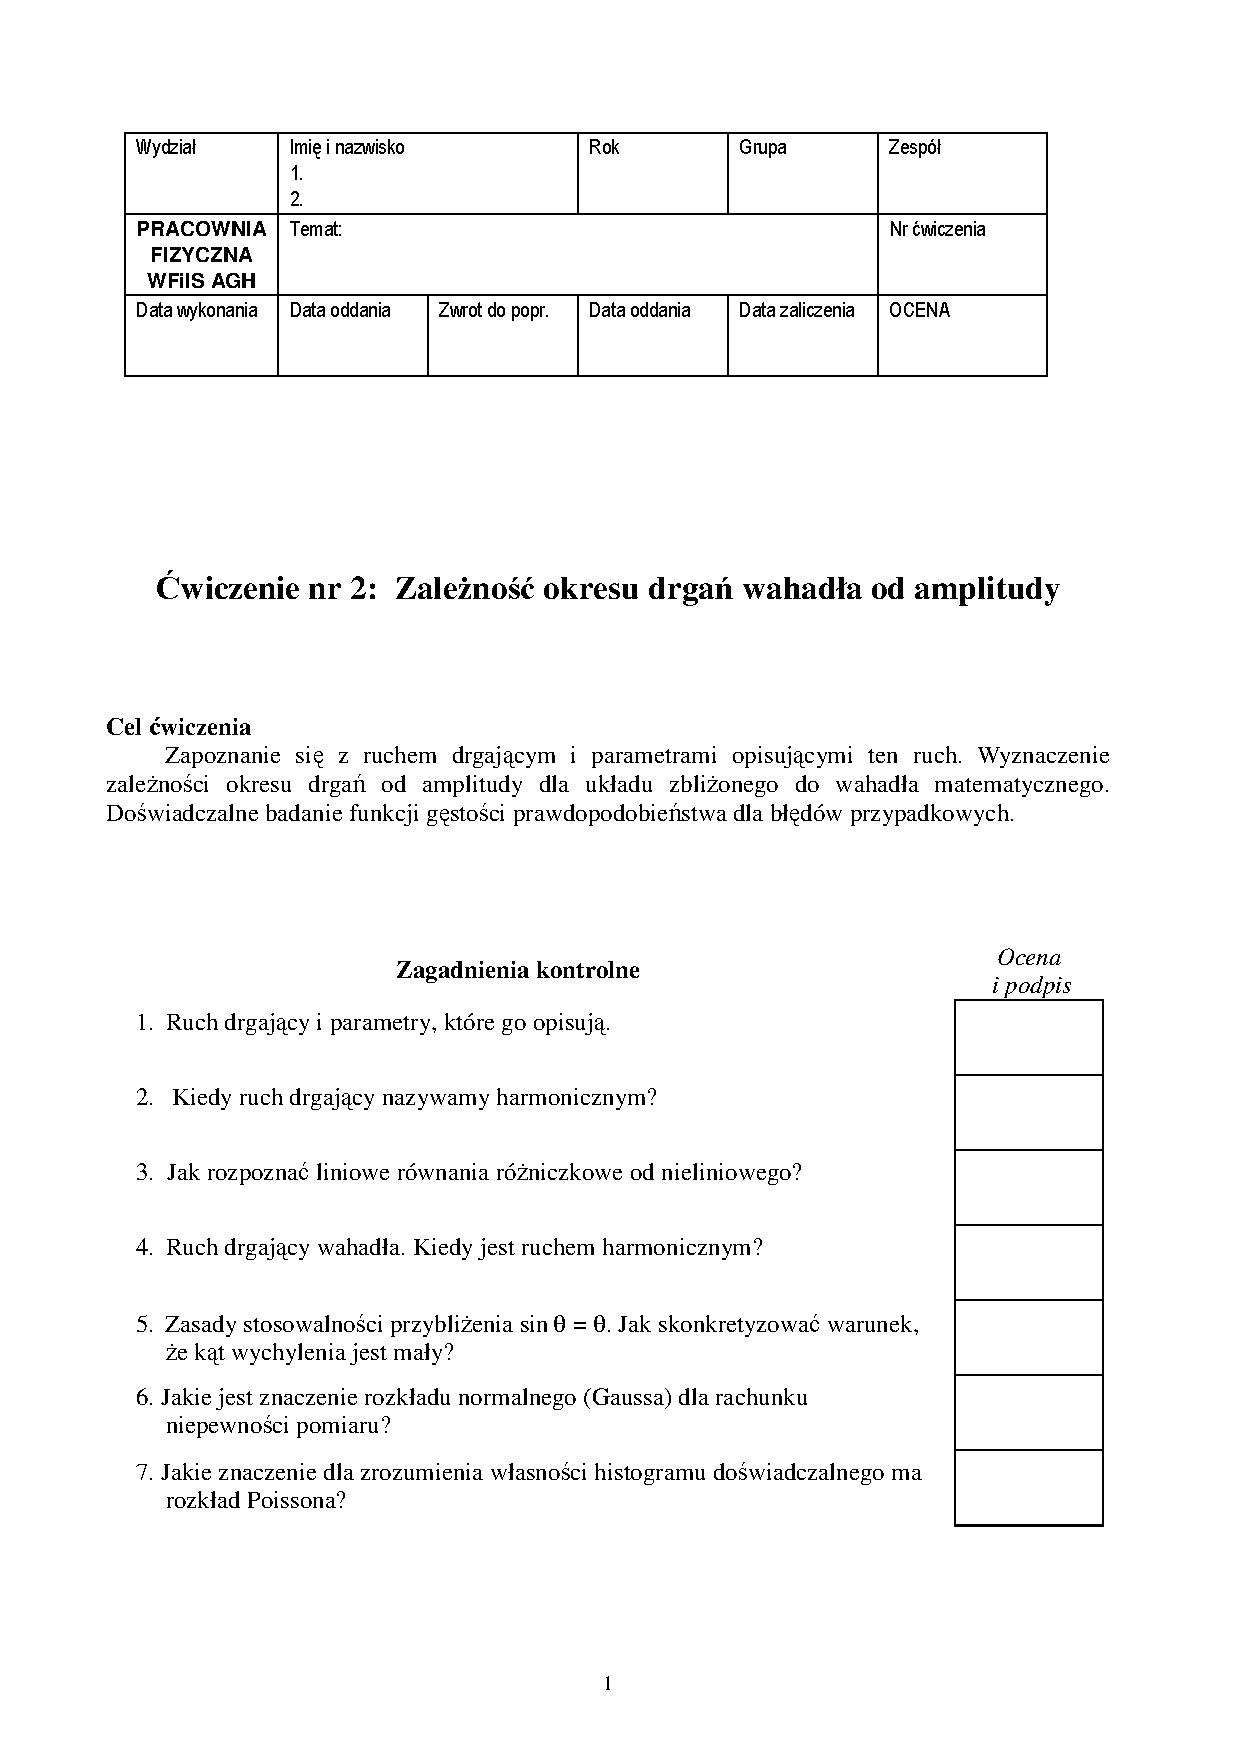
\includepdf[page={2}]{02_wykon}

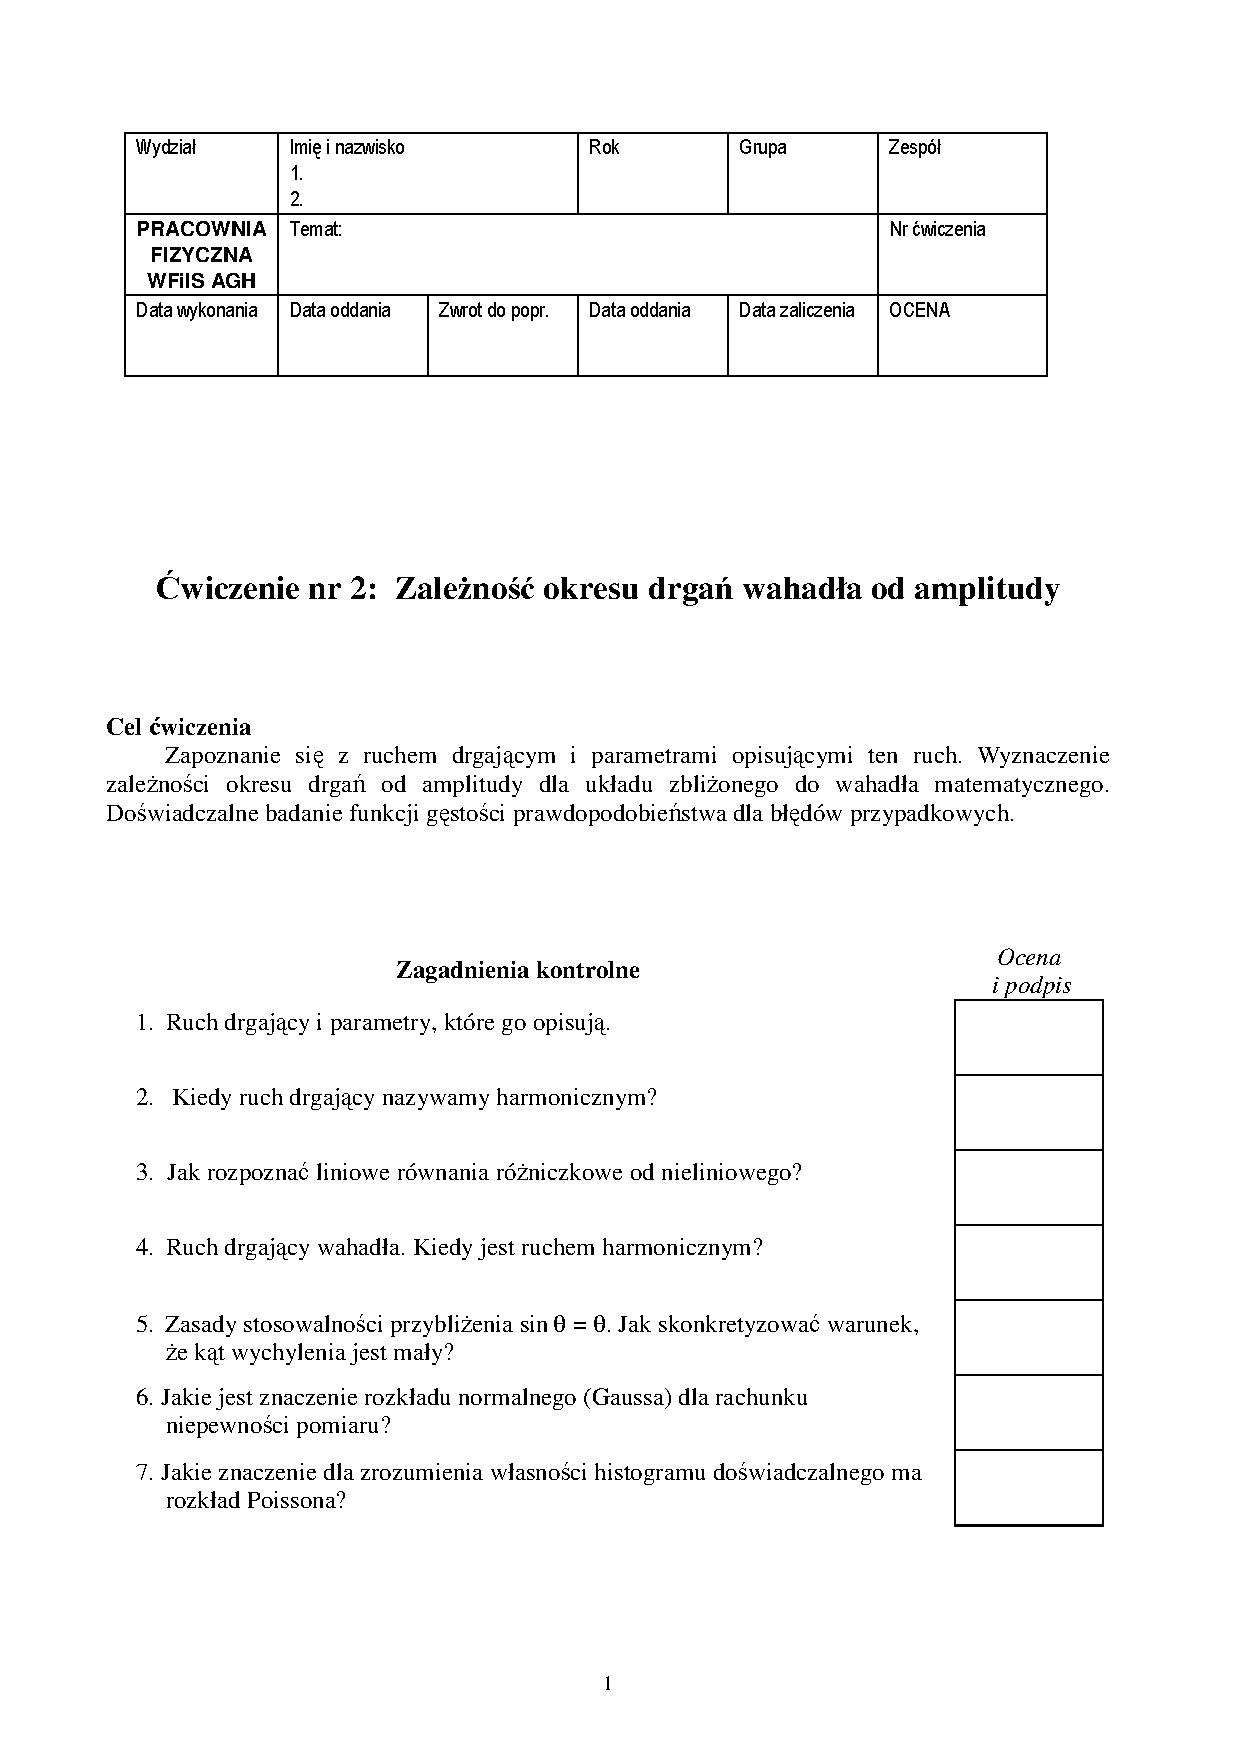
\includepdf[page={5}]{02_wykon}

\begin{justify}
\DIV[3]{section}{Wstęp teoretyczny}
\label{theory}

\subsection{Ruch drgający i parametry, które go opisują}
W ruchu drgającym ciało wychyla się okresowo w jedną i w drugą stronę od położenia równowagi. W położeniu równowagi siły działające na ciało równoważą się.

Wielkości charakteryzujące ruch falowy:
\begin{itemize}
\item amplituda – największe wychylenie z położenia równowagi
\item okres – czas trwania jednego pełnego drgania
\item częstotliwość – ilość drgań zachodzących w ciągu 1 sekundy.
\end{itemize}

\subsection{Kiedy ruch drgający nazywamy harmonicznym?}
Ruch drgający odbywa się, gdy na ciało działa siła proporcjonalna do wychylenia ciała z położenia równowagi (na wykresie wychelenia możemy wtedy zaobserwować krzywą harmoniczną np. sinusoidę).

\subsection{Zasady stosowalności przybliżenia $sin(\theta) = \theta$. Jak skonkretyzować warunek, że kąt wychylenia jest mały? }
O sensowności stosowania przybliżenia $sin(\alpha) = \alpha$ informuje nas różnica pomiędzy sinusem, a wartością kąta w radianach. Poniżej możemy zaobserwować tabelkę, która przedstawia te zależności, dzięki niej możemy wywnioskować, iż przybliżenie ma sens do około 5 - 7 stopni:

\begin{table}[H]
\begin{center}
\begin{scriptsize}
\begin{tabular}{|c|c|c|}
\hline
$\alpha$ & $\alpha$ (rad) & $sin(\alpha)$ \\
\hline
40   &  0,698132 & 0,642788 \\
30   & 0,523599 & 0,500000 \\
20   & 0,349066 & 0,342020 \\
10   & 0,174533 & 0,173648 \\
5    & 0,087266 & 0,087156 \\
2    & 0,034907 & 0,034899 \\
1    & 0,017453 & 0,017452 \\
\hline
\end{tabular}
\end{scriptsize}
\end{center}
\end{table}

\section{Wyniki pomiarów}

\begin{table}[H]
\begin{center}
\begin{scriptsize}
\begin{tabular}{|c|c|c|}
\hline
Liczba okresów k & czas t trwania m okresów [s] & okres T = t/m [s] \\
\hline
40 & 51.503 & 1.287575 \\
40 & 51.826 & 1.29565 \\
40 & 51.598 & 1.28995 \\
40 & 51.792 & 1.2948 \\
40 & 51.748 & 1.2937 \\
\hline
\end{tabular}
\caption{Pomiar okresu $T_{0}$ dla małej amplitudy drgań}
\end{scriptsize}
\end{center}
\end{table}

\begin{table}[H]
\begin{center}
\begin{scriptsize}
\begin{tabular}{|c|c|c|c|c|c|}
\hline
$\theta_{1}$ [$\degree$]  & $\theta_{2}$ [$\degree$]  & mT [s]  & $\frac{(\theta_{1} + \theta_{2})}{2}$ [$\degree$]  & T [s]  & $\frac{T - T_{0}}{T_{0}}$ \\
\hline
5  & 4.0  & 38.612  & 4.50  & 1.287067  & -0.004077 \\
8  & 6.5  & 38.712  & 7.25  & 1.290400  & -0.001497 \\
12  & 10.5  & 38.803  & 11.25  & 1.293433  & 0.000850 \\
15  & 13.5  & 38.874  & 14.25  & 1.295800  & 0.002681 \\
17  & 14.5  & 38.936  & 15.75  & 1.297867  & 0.004280 \\
20  & 17.5  & 38.897  & 18.75  & 1.296567  & 0.003274 \\
23  & 20.5  & 39.049  & 21.75  & 1.301633  & 0.007195 \\
25  & 22.0  & 39.104  & 23.50  & 1.303467  & 0.008614 \\
30  & 26.5  & 39.241  & 28.25  & 1.308033  & 0.012147 \\
\hline
\end{tabular}
\caption{Pomiar zależności okresu od amplitudy }
\end{scriptsize}
\end{center}
\end{table}

\section{Opracowanie wyników}

\subsection{Zależność okresu od średniej amplitudy}

\begin{figure}[h]
\centering
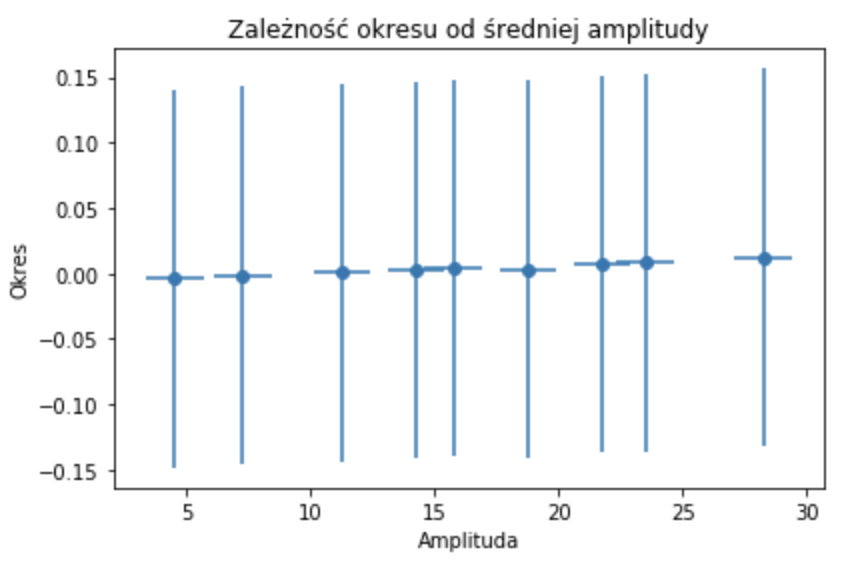
\includegraphics[width=12cm, height=6cm]{okr_ampl}
\end{figure}

\subsection{Pomiary czasu dla małej amplitudy}

\begin{scriptsize}
\begin{longtable}{|c|c|c|}
\hline
$mT_{i}$ [s] & $T_{i}$ [s] & Odchylenie standardowe [s] \\
\hline
3.75 & 1.25 & 0.04293666666666662 \\
3.7569999999999997 & 1.2523333333333333 & 0.040603333333333325 \\
3.765 & 1.2550000000000001 & 0.03793666666666651 \\
3.767 & 1.2556666666666667 & 0.037269999999999914 \\
3.78 & 1.26 & 0.032936666666666614 \\
3.784 & 1.2613333333333332 & 0.03160333333333343 \\
3.7960000000000003 & 1.2653333333333334 & 0.027603333333333202 \\
3.802 & 1.2673333333333334 & 0.0256033333333332 \\
3.802 & 1.2673333333333334 & 0.0256033333333332 \\
3.803 & 1.2676666666666667 & 0.025269999999999904 \\
3.805 & 1.2683333333333333 & 0.02460333333333331 \\
3.806 & 1.2686666666666666 & 0.024270000000000014 \\
3.812 & 1.2706666666666666 & 0.022270000000000012 \\
3.812 & 1.2706666666666666 & 0.022270000000000012 \\
3.813 & 1.2710000000000001 & 0.021936666666666493 \\
3.8169999999999997 & 1.2723333333333333 & 0.020603333333333307 \\
3.823 & 1.2743333333333333 & 0.018603333333333305 \\
3.823 & 1.2743333333333333 & 0.018603333333333305 \\
3.824 & 1.2746666666666666 & 0.01827000000000001 \\
3.8289999999999997 & 1.2763333333333333 & 0.016603333333333303 \\
3.8310000000000004 & 1.2770000000000001 & 0.015936666666666488 \\
3.842 & 1.2806666666666666 & 0.012270000000000003 \\
3.842 & 1.2806666666666666 & 0.012270000000000003 \\
3.843 & 1.281 & 0.011936666666666707 \\
3.844 & 1.2813333333333332 & 0.01160333333333341 \\
3.845 & 1.2816666666666667 & 0.011269999999999891 \\
3.845 & 1.2816666666666667 & 0.011269999999999891 \\
3.8480000000000003 & 1.2826666666666668 & 0.01026999999999978 \\
3.8489999999999998 & 1.283 & 0.009936666666666705 \\
3.85 & 1.2833333333333334 & 0.009603333333333186 \\
3.85 & 1.2833333333333334 & 0.009603333333333186 \\
3.852 & 1.284 & 0.008936666666666593 \\
3.8539999999999996 & 1.2846666666666666 & 0.00827 \\
3.8539999999999996 & 1.2846666666666666 & 0.00827 \\
3.855 & 1.285 & 0.007936666666666703 \\
3.855 & 1.285 & 0.007936666666666703 \\
3.8569999999999998 & 1.2856666666666665 & 0.00727000000000011 \\
3.858 & 1.286 & 0.006936666666666591 \\
3.859 & 1.2863333333333333 & 0.006603333333333294 \\
3.86 & 1.2866666666666666 & 0.006269999999999998 \\
3.865 & 1.2883333333333333 & 0.004603333333333293 \\
3.866 & 1.2886666666666666 & 0.004269999999999996 \\
3.867 & 1.289 & 0.003936666666666699 \\
3.8680000000000003 & 1.2893333333333334 & 0.0036033333333331807 \\
3.8689999999999998 & 1.2896666666666665 & 0.003270000000000106 \\
3.8689999999999998 & 1.2896666666666665 & 0.003270000000000106 \\
3.877 & 1.2923333333333333 & 0.0006033333333332891 \\
3.8789999999999996 & 1.293 & 6.333333333330415e-05 \\
3.8789999999999996 & 1.293 & 6.333333333330415e-05 \\
3.8789999999999996 & 1.293 & 6.333333333330415e-05 \\
3.8810000000000002 & 1.2936666666666667 & 0.0007300000000001194 \\
3.8810000000000002 & 1.2936666666666667 & 0.0007300000000001194 \\
3.885 & 1.295 & 0.002063333333333306 \\
3.886 & 1.2953333333333334 & 0.0023966666666668246 \\
3.887 & 1.2956666666666667 & 0.0027300000000001212 \\
3.89 & 1.2966666666666666 & 0.003730000000000011 \\
3.89 & 1.2966666666666666 & 0.003730000000000011 \\
3.891 & 1.297 & 0.004063333333333308 \\
3.897 & 1.299 & 0.0060633333333333095 \\
3.897 & 1.299 & 0.0060633333333333095 \\
3.897 & 1.299 & 0.0060633333333333095 \\
3.8989999999999996 & 1.2996666666666665 & 0.006729999999999903 \\
3.9 & 1.3 & 0.007063333333333421 \\
3.9019999999999997 & 1.3006666666666666 & 0.007730000000000015 \\
3.903 & 1.301 & 0.008063333333333311 \\
3.903 & 1.301 & 0.008063333333333311 \\
3.904 & 1.3013333333333332 & 0.008396666666666608 \\
3.906 & 1.302 & 0.009063333333333423 \\
3.908 & 1.3026666666666666 & 0.009730000000000016 \\
3.908 & 1.3026666666666666 & 0.009730000000000016 \\
3.91 & 1.3033333333333335 & 0.010396666666666832 \\
3.91 & 1.3033333333333335 & 0.010396666666666832 \\
3.9130000000000003 & 1.3043333333333333 & 0.011396666666666722 \\
3.915 & 1.305 & 0.012063333333333315 \\
3.92 & 1.3066666666666666 & 0.01373000000000002 \\
3.9219999999999997 & 1.3073333333333332 & 0.014396666666666613 \\
3.9219999999999997 & 1.3073333333333332 & 0.014396666666666613 \\
3.923 & 1.3076666666666668 & 0.014730000000000132 \\
3.924 & 1.308 & 0.015063333333333428 \\
3.925 & 1.3083333333333333 & 0.015396666666666725 \\
3.925 & 1.3083333333333333 & 0.015396666666666725 \\
3.925 & 1.3083333333333333 & 0.015396666666666725 \\
3.927 & 1.309 & 0.01606333333333332 \\
3.931 & 1.3103333333333333 & 0.017396666666666727 \\
3.9330000000000003 & 1.3110000000000002 & 0.018063333333333542 \\
3.935 & 1.3116666666666668 & 0.018730000000000135 \\
3.9360000000000004 & 1.312 & 0.019063333333333432 \\
3.937 & 1.3123333333333334 & 0.01939666666666673 \\
3.938 & 1.3126666666666666 & 0.019730000000000025 \\
3.94 & 1.3133333333333332 & 0.02039666666666662 \\
3.943 & 1.3143333333333334 & 0.02139666666666673 \\
3.945 & 1.315 & 0.022063333333333324 \\
3.9539999999999997 & 1.3179999999999998 & 0.025063333333333215 \\
3.966 & 1.322 & 0.02906333333333344 \\
3.971 & 1.3236666666666668 & 0.030730000000000146 \\
3.9760000000000004 & 1.3253333333333335 & 0.03239666666666685 \\
3.992 & 1.3306666666666667 & 0.03773000000000004 \\
3.997 & 1.3323333333333334 & 0.039396666666666746 \\
4.013999999999999 & 1.3379999999999999 & 0.04506333333333323 \\
4.016 & 1.3386666666666667 & 0.04573000000000005 \\
\hline
\caption{Pomiar zależności okresu od amplitudy }
\end{longtable}
\end{scriptsize}

\begin{figure}[h]
\centering
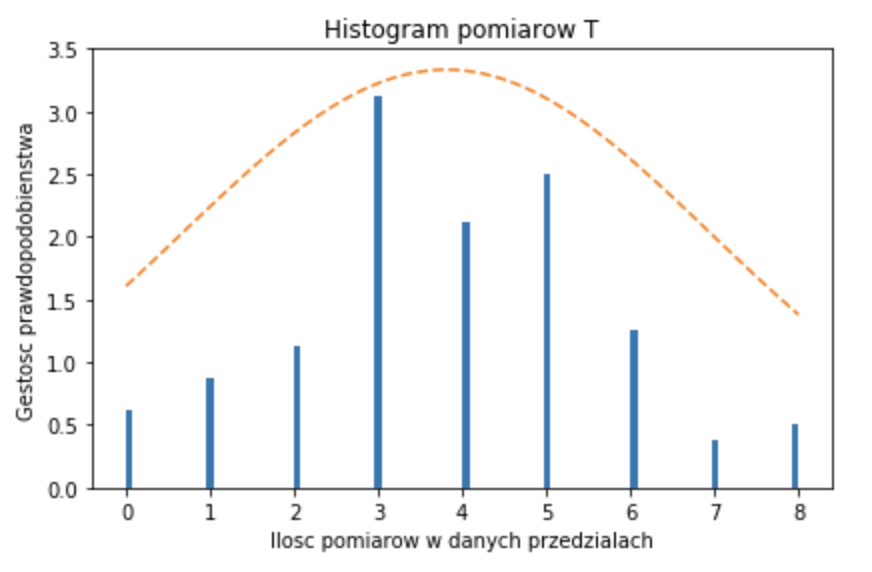
\includegraphics[width=12cm, height=6cm]{gauss}
\end{figure}

\section{Bibliografia}

\begingroup
\renewcommand{\section}[2]{}%
\begin{thebibliography}{}
\bibitem{instrukcja} \url{http://www.fis.agh.edu.pl/~pracownia_fizyczna/cwiczenia/02_wykon.pdf}
\end{thebibliography}
\endgroup

\end{justify}

\end{document}